\newpage
\section{Instructions: Language of the Machine}
The process of compiling:
\begin{enumerate}
    \item High-level programming language
    \item Assembly language
    \item Machine language
\end{enumerate}

\subsection{Introduction}
Language of the machine: \begin{itemize}
    \item\small Instructions -> words
    \item\small Instructions set -> vocabulary
\end{itemize}

Chosen: RISC-V

\subsubsection{Instruction Set}

CISC vs RISC

\begin{table}[!htb]
    \centering
    \caption{CISC vs RISC}
    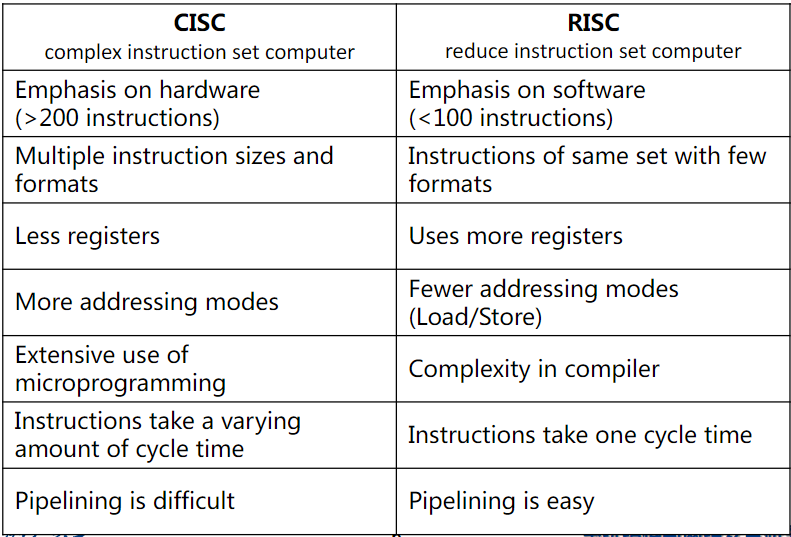
\includegraphics[width=0.479\textwidth]{CO3/CISC vs RISC}
\end{table}


% \begin{table*}[htb]
%     \centering
%     \caption{CISC vs RISC}
%     \begin{tabular}[c]{|p{16em}|p{16em}|}\hline
%         \makecell{CISC\\  \small complex instruction set computer}  & \makecell{RISC \\  reduce instruction set computer} \\\hline
%         \makecell[l]{Emphasis on hardware\\>200 instruction} & \makecell[l]{Emphasis on hardware\\<100 instruction}   \\ \hline
%         Multiple instruction sizes and formats & Instructions of same set with few formats \\ \hline
%         Less registers & Uses more registers\\ \hline
%         More addressing modes & Fewer addressing modes (Load/Store) \\  \hline
%         Extensive use of microprogramming & Complexity in compiler \\ \hline
%         Instructions take a varying amount of cycle time & Instructions take one cycle time \\ \hline
%         Pipelining is difficult & Pipelining is easy \\ \hline
%     \end{tabular}
% \end{table*}

\subsubsection{Instruction formats}
\begin{figure}[!htb]
    \centering
    \begin{tikzpicture}
        \node (op) at (0,0) [rectangle, draw=light_blue, text width=4.5em, text centered] {\textcolor{light_red}{Op}};
        \node (opd) [right=0em of op] [rectangle, draw=light_blue, text width=7em, text centered] {\textcolor{light_red}{Operands}};
        \node [above=0em of op] {Operators};
        \node [above=0.2em of opd] {wide variety};

        \draw [black] (1.2,0.3)--(1.2,0.5)--(3.6,0.5)--(3.6,0.3);
    \end{tikzpicture}
\end{figure}
Type of internal storage in processer. 
The number of the memory operand In the instruction. 

\subsubsection{Stored-program concept}
Today's computers are built on 2 key principles (Stored-program concept): 
\begin{enumerate}
    \item Instruction are represented as numbers.
    \item Programs can be stored in memory to be read or written just like numbers.
\end{enumerate}

\subsection{Arithmetic Operations}
Every computer should perform arithmetic. Only one operation per instruction (Two sources and one destination). 
All arithmetic operations have this form. 

Design Principle 1: Simplicity favors regularity. Regularity makes implementation simpler. Simplicity enables higher performance at lower cost

\subsubsection{Arithmetic Example}
\begin{lstlisting}[language=c, title={C code}]
f=(g+h)-(i+j);
\end{lstlisting}

\begin{lstlisting}[language={[x86masm]Assembler}, title={Compiled RISC-V code}]
add t0, g, h
add t1, i, j
sub f, t0, t1
\end{lstlisting}

% \begin{table}[!htb]
%     \centering
%     \caption{RISC-V assembly language}
%     \begin{tabular}[c]{|c|c|c|c|}\hline
%         Category & Instruction & Example & Meaning\\ \hline
%         \multirow{2}{5em}{Arithmetic} & add & add a,b,c & a$\leftarrow$b+c\\ \cline{2-4}
%         & substract & sub a,b,c & a$\leftarrow$b-c\\ \hline
%     \end{tabular}
% \end{table}


\subsection{Operands}
Arithmetic instructions use register operands. RISC-V has a 32 $\times$ 64-bit register file. Use for frequently accessed data. 64-bit data is called a ``doubleword''. 32 x 64-bit general purpose registers x0 to x31. 32-bit data is called a ``word''. 

Design Principle 2: Smaller is faster. c.f. main memory: millions of locations

\subsubsection{RISC-V Registers}

\begin{figure}[!htb]
    \centering
    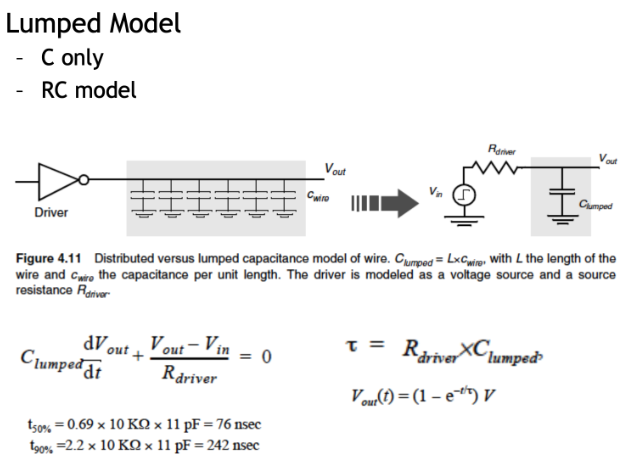
\includegraphics[width=0.489\textwidth]{CO3/RISC-V Registers}
    \caption{RISC-V Registers}
\end{figure}

\begin{table}[!htb]
    \centering
    \caption{RISC-V Registers table}
    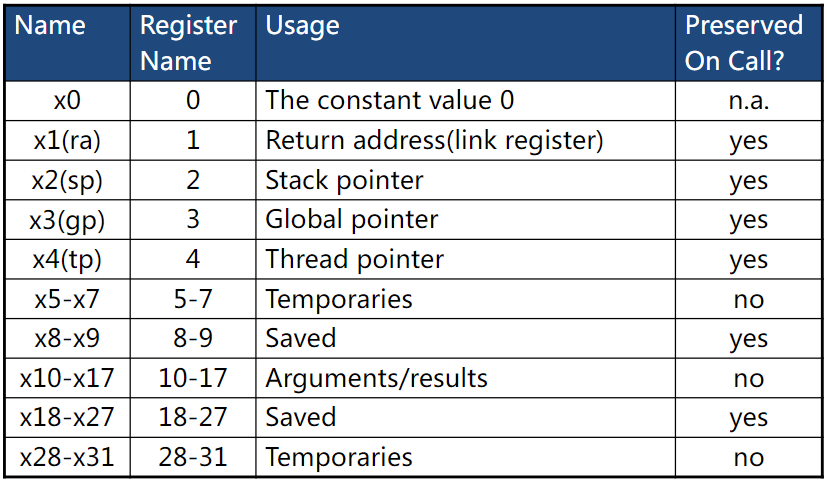
\includegraphics[width=0.479\textwidth]{CO3/RISC-V Registers table}
\end{table}


\subsubsection{Register Operand Example}
\begin{lstlisting}[language={C},title={C code}]
f = (g + h) - (i + j);
\end{lstlisting}
f, g, h, i, j in x19, x20, x21, x22, x23. 

\begin{lstlisting}[language={[x86masm]Assembler},title={Compiled RISC-V code}]
add x5, x20, x21
add x6, x22, x23
sub x19, x5, x6
\end{lstlisting}


\subsubsection{Memory Operands}
Main memory used for composite data e.g. Arrays, structures, dynamic data. 
To apply arithmetic operations: 
\begin{itemize}
    \item\small Load values from memory into registers
    \item\small Store result from register to memory
\end{itemize}

Memory is byte addressed. Each address identifies an 8-bit byte. 

RISC-V is Little Endian. Least-significant byte at least address of a word. c.f. Big Endian: most-significant byte at least address

RISC-V does not require words to be aligned in memory, unlike some other ISAs. 

\subsubsection{Memory Alignment}
\begin{lstlisting}[language=c]
struct {
    int a;
    char b;
    char c[2];
    char d[3];
    float e;
}
\end{lstlisting}

\begin{table}[!htb]
    \centering
    \begin{tabular}[c]{|c|c|c|c|}\hline
        \multicolumn{4}{|c|}{e}\\ \hline
        d[1] & d[2] & No use & No use \\ \hline
        b & c[0] & c[1] & d[0] \\ \hline
        \multicolumn{4}{|c|}{a}\\ \hline
    \end{tabular}
\end{table}


因为一次只能读出4字节内存中的一行, 如此e变量能一次读出. 

\subsubsection{Endianness/byte order}
Big end: Leftmost e.g. PowerPC 01 02 = 258. 

Little end: Rightmost e.g. RISC-V 01 02 = 513. 

\begin{figure}[!htb]
    \centering
    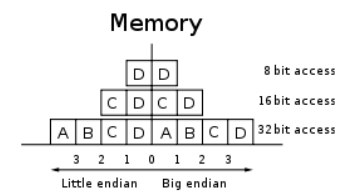
\includegraphics[width=0.479\textwidth]{CO3/Endianness}
    \caption{Endianness}
\end{figure}

\subsubsection{Memory Operand Example}
\begin{lstlisting}[language={C},title={C code}]
A[12]=h+A[8]
\end{lstlisting}
h in x21, base address of A in x22. 

\begin{enumerate}
    \item Index 8 requires offset of 64, 8 bytes per doubleword. 
    \item  Offset: the constant in a data transfer instruction. 
    \item  Base register: the register added to form the address. 
\end{enumerate}
\begin{lstlisting}[language={[x86masm]Assembler},title={Compiled RISC-V code}]
ld x9, 64(x22)
add x9, x21, x9
sd x9, 96(x22)
\end{lstlisting}
ld means load double word, lw means load word. Same sd means save double word. 

\subsubsection{Register vs Memory}
Registers are faster to access than memory. Compiler must use registers for variables as much as possible. Only spill to memory for less frequently used variables. 

\subsubsection{Constant or immediate Operands (立即数)}
Avoids the load instruction. 
\begin{lstlisting}[language={[x86masm]Assembler},title={Compiled RISC-V code}]
addi x22, x22, 4 // x22=x22+4
\end{lstlisting}
Constant zero: a register x0. 

Design Principle 3: Make common case fast. 

\subsubsection{Brief summary}

\begin{table}[!htb]
    \centering
    \caption{RISC-V assembly language}
    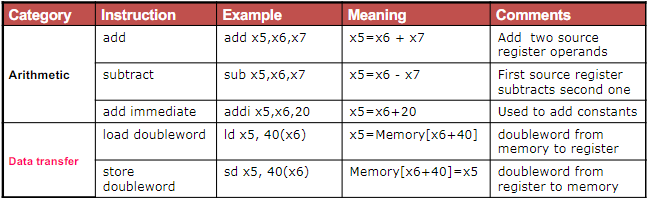
\includegraphics[width=0.489\textwidth]{CO3/RISC-V assembly language-1}
\end{table}

\begin{table}[!htb]
    \centering
    \caption{RISC-V operands}
    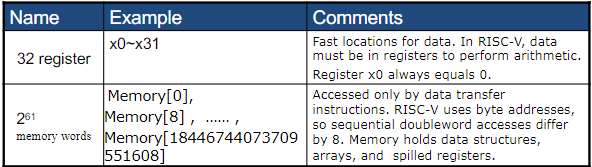
\includegraphics[width=0.489\textwidth]{CO3/RISC-V operands}
\end{table}

\subsection{Signed and unsigned numbers}
In RISC-V instruction set
\begin{itemize}
    \item lb: sign-extend loaded byte
    \item lbu: zero-extend loaded byte
\end{itemize}

\subsection{Representing Instructions}
RISC-V instructions: 
\begin{itemize}
    \item Encoded as 32-bit instruction words
    \item Small number of formats encoding operation code (opcode), register numbers, ...
    \item Regularity
\end{itemize}

\subsubsection{Example: Translating Assembly Code}
\begin{lstlisting}[language={[x86masm]Assembler},title={Compiled RISC-V code}]
add x9, x20, x21
\end{lstlisting}

Decimal version of machine code
\begin{table}[!htb]
    \centering
    \begin{tabular}[c]{|c|c|c|c|c|c|}\hline
        0 & 21 & 20 & 0 & 9 &51 \\ \hline
    \end{tabular}
\end{table}

Binary version of machine code
\begin{table}[!htb]
    \centering
    \begin{tabular}[c]{|c|c|c|c|c|c|}\hline
        0000000 & 10101 & 10100 & 000 & 01001 & 0110011 \\ \hline
        7 bits & 5 bits & 5 bits & 3 bits & 5 bits &7 bits \\ \hline
    \end{tabular}
\end{table}


\subsubsection{Hexadecimal}
Base 16: Compact representation of bit strings, 4 btis pre hex digit. 

e.g. eca8 6420: 1110 1100 1010 1000 0110 0100 0010 0000

可以打表记指令
\subsubsection{RISC-V R-Format Instructions (R型指令)}
\begin{table}[!htb]
    \centering
    \begin{tabular}[c]{|c|c|c|c|c|c|}\hline
        fnuct7 & rs2 & rs1 & funct3 & rd & opcode \\ \hline
        7 bits & 5 bits & 5 bits & 3 bits & 5 bits &7 bits \\ \hline
    \end{tabular}
\end{table}

Instruction fields:
\begin{itemize}
    \item opcode: operation code
    \item rd: destination register number
    \item funct3: 3-bit function code (additional opcode)
    \item rs1: the first source register number
    \item rs2: the second source register number
    \item funct7: 7-bit function code (additional opcode)
\end{itemize}
All instructions in RISC-V have the same length. 

\subsubsection{RISC-V I-Format Instructions (I型指令)}
\begin{table}[!htb]
    \centering
    \begin{tabular}[c]{|c|c|c|c|c|}\hline
        immediate & rs1 & funct3 & rd & opcode \\ \hline
        12 bits & 5 bits & 3 bits & 5 bits &7 bits \\ \hline
    \end{tabular}
\end{table}

Immediate arithmetic and load instructions:
\begin{itemize}
    \item rs1: source or base address register number
    \item immediate: constant operand, or offset added to base address, e.g. 2s-complement, sign extended
\end{itemize}

e.g. ld x9, 64(x22)
\begin{itemize}
    \item 22 (x22) is placed rs1
    \item 64 is placed immediate
    \item 9 (x9) is placed rd
\end{itemize}

\subsubsection{RISC-V S-Format Instructions (S型指令)}

\begin{table}[!htb]
    \centering
    \begin{tabular}[c]{|c|c|c|c|c|c|}\hline
        \small imm[11:5] & rs2 & rs1 & funct3 & \small imm[4:0] & opcode \\ \hline
        7 bits & 5 bits & 5 bits & 3 bits & 5 bits &7 bits \\ \hline
    \end{tabular}
\end{table}

Different immediate format for store instructions
\begin{itemize}
    \item rs1: base address register number
    \item rs2: source operand register number
    \item immediate: offset added to base address. Split so that rs1 and rs2 fields always in the same place. 
\end{itemize}

e.g. sd x9, 64(x22)
\begin{itemize}
    \item 22 (x22) is placed rs1
    \item 64 is placed immediate
    \item 9 (x9) is placed rs2
\end{itemize}

\subsubsection{RISC-V instruction encoding}
\begin{table}[!htb]
    \centering
    \caption{RISC-V instruction encoding}
    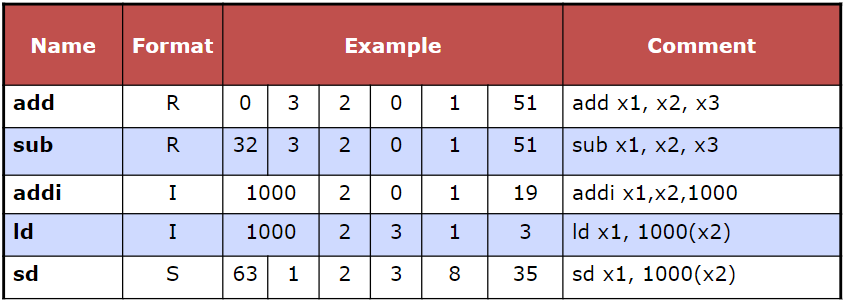
\includegraphics[width=0.39\textwidth]{CO3/RISC-V instruction encoding-1}
\end{table}

Two key principles of today's computers:
\begin{enumerate}
    \item Instructions are represented as numbers (Stred-program)
    \item Programs can be stored in memory like numbers 
\end{enumerate}

\subsubsection{RISC-V fields (format)}
\begin{table}[!htb]
    \centering
    \caption{RISC-V fields (format)}
    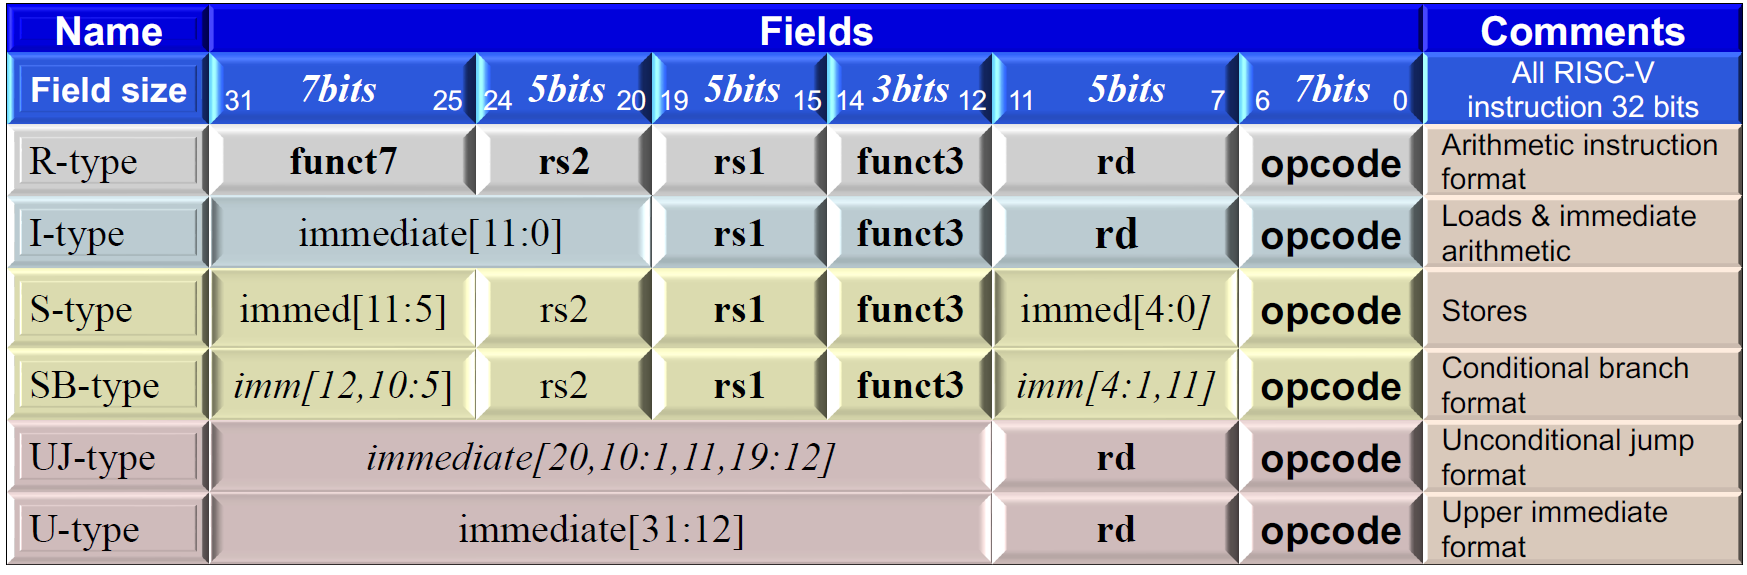
\includegraphics[width=0.489\textwidth]{CO3/RISC-V fields (format)}
\end{table}

\subsubsection{Stored Program Computer}
Before, the program is stored as data. 
Future, the data may be the model.


\subsection{Logical operations}
\begin{table}[!htb]
    \centering
    \caption{Instructions for bitwise manipulation}
    \begin{tabular}[c]{|l|c|c|c|}\hline
        \makecell[c]{Operation} & C & Java & RISC-V\\ \hline
        Shift left & $<<$ & $<<$ &  slli \\ \hline
        Shift right& $>>$ & $>>$ & srli \\ \hline
        Bit-by-bit AND & \& & \& & and, andi \\ \hline
        Bit-by-bit OR & | & | & or, ori\\ \hline
        Bit-by-bit XOR & \^{} & \^{} & xor, xori\\ \hline
        Bit-by-bit NOT & $\sim$ & $\sim$ & \\ \hline
    \end{tabular}
\end{table}
Useful for extracting and inserting groups of bits in a word. 

\subsubsection{Shift Operations}
\begin{table}[!htb]
    \centering
    \begin{tabular}[c]{|c|c|c|c|c|c|}\hline
        funct6 & immed & rs1 & funct3 & rd & opcode \\ \hline
        6 bits & 6 bits & 5 bits & 3 bits & 5 bits &7 bits \\ \hline
    \end{tabular}
\end{table}
immed: how many positions to shift. 

\subsubsection{AND Operations}
Useful to mask bits in a word. Select some bits, clear others to 0. 

\subsubsection{OR Operations}
Useful to include bits in a word. Set some bits to 1, leave others unchanged. 

\subsubsection{XOR Operations}
Differencing operation. Set some bits to 1, leave others unchanged. 

\begin{table}[!htb]
    \centering
    \caption{RISC-V assembly language}
    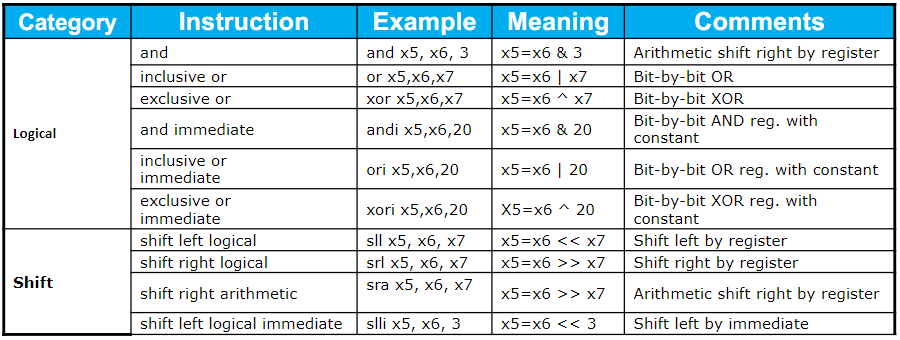
\includegraphics[width=0.489\textwidth]{CO3/RISC-V assembly language-2}
\end{table}


\subsection{Instructions for making decision}
Branch instructions: Branch to a labeled instruction if a condition is true. Otherwise, continue sequentially. 

\begin{lstlisting}[language={[x86masm]Assembler}]
beq rs1, rs2, L1 
\end{lstlisting}
If (rs1 == rs2) branch to instruction labeled L1

\begin{lstlisting}[language={[x86masm]Assembler}]
bne rs1, rs2, L1 
\end{lstlisting}
If (rs1 != rs2) branch to instruction labeled L1

\subsubsection{Example Compiling an if statement}
Assume: f $\sim$ j --- x19 $\sim$ x23
\begin{lstlisting}[language={c},title={C code}]
if ( i == j ) goto L1 ;
f = g + h ;
L1: f = f - i ;
\end{lstlisting}

\begin{lstlisting}[language={[x86masm]Assembler},title={RISC-V assembly code}]
beq x21, x22, L1
add x19, x20, x21
L1: sub x19, x19, x22
\end{lstlisting}
\begin{enumerate}
    \item go to L1 if i equals j
    \item f = g + h (skipped if i equals j)
    \item f = f - i (always executed)
\end{enumerate}

\subsubsection{Compiling if-then-else}
Assume: f $\sim$ j --- x19 $\sim$ x23
\begin{lstlisting}[language={c},title={C code}]
if ( i == j ) f = g + h ;
else f = g - h ;
\end{lstlisting}

\begin{lstlisting}[language={[x86masm]Assembler},title={RISC-V assembly code}]
bne x22, x23, Else
add x19, x20, x21
beq x0, x0, EXIT
Else: sub x19, x20, x21
Exit: ...... statement
\end{lstlisting}
\begin{enumerate}
    \item go to Else if i != j
    \item f = g + h ( Executed if i == j if)
    \item go to Exit
    \item f = g - h ( Executed if i != j else)
    \item the first instruction of the next C
\end{enumerate}

\subsubsection{Compiling LOOPs}
Assume: g $\sim$ j --- x19 $\sim$ x23 base of A[i] --- x25
\begin{lstlisting}[language={c},title={C code}]
Loop: 
    g = g + A[i] ; // A is an array of 100 words
    i = i + j ;
    if ( i != h ) goto Loop ;
\end{lstlisting}

\begin{lstlisting}[language={[x86masm]Assembler},title={RISC-V assembly code}]
Loop: 
    slli x10, x22, 3
    add x10, x10, x25 
    ld x19, 0(x10)
    add x20, x20, x19 
    add x22, x22, x23 
    bne x22, x21, Loop
\end{lstlisting}
\begin{enumerate}
    \item  temp reg x10 = 8 * i
    \item x10 = address of A[i]
    \item temp reg x19 = A[i]
    \item g = g + A[i]
    \item i = i + j
    \item go to Loop if i != h
\end{enumerate}

\subsubsection{Compiling while}
Assume: i $\sim$ k --- x22 and x24 base of save --- x25
\begin{lstlisting}[language={c},title={C code}]
while ( save[i] == k )
    i = + i ;
\end{lstlisting}

\begin{lstlisting}[language={[x86masm]Assembler},title={RISCV assembly code}]
Loop: 
    slli x10, x22, 3
    add x10, x10, x25 
    ld x9, 0(x10)     
    bne x9, x24, Exit 
    addi x22, x22, 1
    beq x0, x0, Loop
Exit:
\end{lstlisting}
\begin{enumerate}
    \item  temp reg \$t1 = 8 * i
    \item x10 = address of save[i]
    \item x9 gets save[i]
    \item go to Exit if save[i] != k
    \item i += 1
    \item go to Loop
\end{enumerate}

\subsubsection{More Conditional Operations}
\begin{lstlisting}[language={[x86masm]Assembler}]
blt rs1, rs2, L1
\end{lstlisting}
if (rs1 < rs2) branch to instruction labeled L1
\begin{lstlisting}[language={[x86masm]Assembler}]
bge rs1, rs2, L1
\end{lstlisting}
if (rs1 >= rs2) branch to instruction labeled L1

\subsubsection{Signed vs. Unsigned}
\begin{itemize}
    \item\small Signed comparison: blt, bge. 
    \item\small Unsigned comparison: bltu, bgeu. 
\end{itemize}

\subsubsection{Hold out Case/Switch}
Used to select one of many alternatives. Compiling a switch using jump address table. 

Assume: f $\sim$ k --- x20 $\sim$ x25 x5 contains 4/8
\begin{lstlisting}[language={c},title={C code}]
switch ( k ) {
    case 0 : f=i+j; break; /* k=0 */
    case 1 : f=g+h; break; /* k=1 */
    case 2 : f=g-h; break; /* k=2 */
    case 3 : f=i-j; break; /* k=3 */
}
\end{lstlisting}

\begin{lstlisting}[language={[x86masm]Assembler},title={RISC-V assembly code}]
blt x25, x0, Exit
bge x25, x5, Exit
slli x7, x25, 3
add x7, x7, x6 
ld x7, 0(x7)
jalr x1, 0(x7) 
\end{lstlisting}
\begin{enumerate}
    \item test if k < 0
    \item if k >= 4, go to Exit
    \item temp reg x7 = 8 * k (0<=k<=3)
    \item x7 = address of JumpTable[k]
    \item temp reg x7 gets JumpTable[k]
    \item jump based on register x7(entrance)
\end{enumerate}

jump address table: x7=x6+8*k
\begin{lstlisting}[language={[x86masm]Assembler},title={Memory1}]
L0: address
L1: address
L2: address
L3: address
\end{lstlisting}
\begin{lstlisting}[language={[x86masm]Assembler},title={Memory2}]
L0: 
    add $s0, $s3, $s4
    jalr x0, 0(x1)
L1: 
    add $s0, $s1, $s2
    jalr x0, 0(x1)
L2: 
    sub $s0, $s1, $s2
    jalr x0, 0(x1)
L3: 
    sub $s0, $s3, $s4
    jalr x0, 0(x1)
\end{lstlisting}
\begin{itemize}
    \item L0
    \begin{enumerate}
        \item k = 0 so f gets i + j
        \item end of this case so go to Exit
    \end{enumerate}
    \item L1
    \begin{enumerate}
        \item k = 1 so f gets g + h
        \item end of this case so go to Exit
    \end{enumerate}
    \item L2
    \begin{enumerate}
        \item k = 2 so f gets g - h
        \item end of this case so go to Exit
    \end{enumerate}
    \item L3
    \begin{enumerate}
        \item k = 3 so f gets i - j
        \item end of this case so go to Exit
    \end{enumerate}
\end{itemize}



\subsubsection{Jump register \& jump address table}
Jump with register content
\begin{lstlisting}[language={[x86masm]Assembler}]
jalr x1, 100(x6)
\end{lstlisting}

Jump address table: x7 $\leftarrow$ x6 + 4/8*K

% 画个图在者, P57

\subsubsection{Important conception --- Basic Blocks}
A basic block is a sequence of instructions with 
\begin{itemize}
    \item\small No embedded branches (except at end)
    \item\small No branch targets (except at beginning)
\end{itemize}

A compiler identifies basic blocks for optimization. An advanced processor can accelerate execution of basic blocks. 

\subsection{Supporting procedures}
Procedure/function be used to structure programs. A stored subroutine that performs a specific task based on the parameters with which it is provided, easier to understand, allow code to be reused. 
\begin{enumerate}
    \item Place Parameters in a place where the procedure can access
    them
    \item Transfer control to the procedure: jump to
    \item Acquire the storage resources needed for the procedure
    \item Perform the desired task
    \item Place the result value in a place where the calling program can access it
    \item Return control to the point of origin
\end{enumerate}

\subsubsection{Procedure Call Instructions}
\begin{itemize}
    \item Instruction for procedures: \hl{jal} ( jump-and-link )
    \begin{lstlisting}[language={[x86masm]Assembler}, title={Caller}]
jal x1, ProcedureAddress
    \end{lstlisting}
    \begin{enumerate}
        \item Address of following instruction put in x1 (PC+4 $\rightarrow$ ra).
        \item Jumps to target address. 
    \end{enumerate}
    
    \item Procedure return: \hl{jalr} (jump and link register)
    \begin{lstlisting}[language={[x86masm]Assembler}, title={Callee }]
jalr x0, 0(x1)
    \end{lstlisting}
    \begin{enumerate}
        \item Like jal, but jumps to 0 + address in x1.
        \item Use x0 as rd (x0 cannot be changed). 
    \end{enumerate}
    Can also be used for computed jumps. 
     
\end{itemize}

\subsubsection{Using More Registers}
More Registers for procedure calling: 
\begin{itemize}
    \item\small a0 $\sim$ a7(x10-x17): eight argument registers to pass parameters \& return values
    \item\small ra/x1: one return address register to return to origin point
\end{itemize}

Stack: ideal data structure for spilling registers. push, pop and Stack pointer (sp). 

Stack grow from higher address to lower address. 
\begin{itemize}
    \item\small Push: sp= sp - 8
    \item\small Pop: sp = sp + 8
\end{itemize}

e.g. Compiling a leaf procedure ( Assume: g, ..., j in x10, ..., x13 and f in x20)

\begin{lstlisting}[title={C code}]
ll leaf(ll g, ll h, ll i, ll j){
    ll f;
    f = (g + h) - (i + j);
    return f;
}
\end{lstlisting}

\begin{lstlisting}[language={[x86masm]Assembler},title={RISC-V assembly code}]
addi sp, sp, -24
sd x5, 16(sp)
sd x6, 8(sp)
sd x20, 0(sp)

add x5, x10, x11
add x6, x12, x11
sub x20, x5, x6
addi x10, x20 ,0
    
ld x20, 0(sp)
ld x6, 8(sp)
ld x5, 16(sp)
addi sp, sp, +24
jalr x0, 0(x1)
\end{lstlisting}
\begin{itemize}
    \item PUSH
    \begin{enumerate}
        \item  adjust stack to make room for 3 items. 
        \item These three instructions save three register x5, x6 (Save value), x20 (Return value). 
    \end{enumerate}
    \item LEAF
    \begin{enumerate}
        \item register x5 contains g + h
        \item register x6 contains i + j
        \item f = x5- x6, which is ( g + h ) – ( i + j )
        \item copy f to return register (x10 = x20 + 0)
    \end{enumerate}
    \item POP
    \begin{enumerate}
        \item restore register x20 for caller
        \item restore register x6 for caller
        \item restore register x5 for caller
        \item adjust stack to delete 3 items
        \item jump back to calling routine
    \end{enumerate}
\end{itemize}

But maybe some of the three are not used by the caller. So, this way might be inefficient to save x5, x6, x20 on stack. Two classes of registers
\begin{itemize}
    \item\small t0 $\sim$ t6: 7 temporary registers, by the callee not preserved
    \item\small s0 $\sim$ s11: 12 saved registers, must be preserved If used
\end{itemize}

\begin{figure}[!htb]
    \centering
    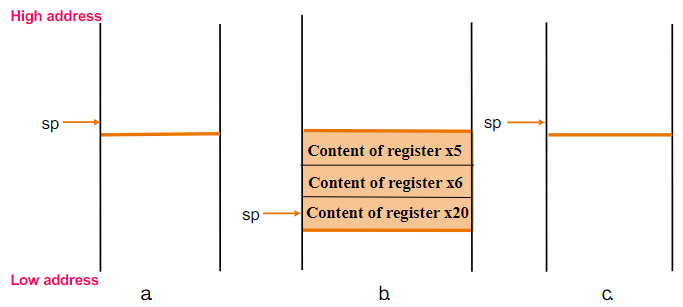
\includegraphics[width=0.489\textwidth]{CO3/The values of the stack pointer and stack before, during and after procedure call}
    \caption{The values of the stack pointer and stack before, during and after procedure call}
\end{figure}

Conflict over the use of register both. Push all the registers to stack. 
\begin{itemize}
    \item\small Caller: pushes a0$\sim$a7 or t0$\sim$t6
    \item\small Callee: pushes ra (return address) and s0$\sim$s11
\end{itemize}


\subsubsection{Nested Procedures}
Compiling a recursive procedure ( Assume: n --- a0 )
\begin{lstlisting}[language={c},title={C code for n!}]
int fact(int n){
    if(n<1)return 1;
    else return n*fact(n-1);
}
\end{lstlisting}

\begin{lstlisting}[language={[x86masm]Assembler},title={RISC-V assembly code}]
fact:
    addi sp, sp, -16
    sd ra, 8(sp)
    sd a0, 0(sp)
    addi t0, a0, -1
    bge t0, zero, L1
    addi a0, zero, 1
    addi sp, sp, 16
    jalr zero, 0(ra)
L1: 
    addi a0, a0, -1
    jal ra, fact
    addi t1, a0, zero
    ld a0, 0(sp)
    ld ra, 8(sp)
    addi sp, sp, 16
    mul a0, a0, t1
    jalr zero, 0(ra)
\end{lstlisting}
\begin{itemize}
    \item fact
    \begin{enumerate}
        \item adjust stack for 2 items
        \item save the return address: x1
        \item save the argument n: x10
        \item x5 = n - 1
        \item if n >= 1, go to L1(else)
        \item return 1 if n <1
        \item Recover sp
        \item return to caller
    \end{enumerate}
    \item L1
    \begin{enumerate}
        \item  n >= 1: argument gets ( n - 1 )
        \item call fact with ( n - 1)
        \item move result of fact(n - 1) to x6(t1)
        \item return from jal: restore argument n
        \item restore the return address
        \item adjust stack pointer to pop 2 items
        \item return n*fact ( n - 1 )
        \item return to the caller
    \end{enumerate}
\end{itemize}

Preserved things across a procedure call. 
\begin{itemize}
    \item\small Saved registers(s0 $\sim$ s11), stack pointer register(\$sp),
    \item\small return address register(ra/x1), stack \textbf{above} the stack pointer. 
\end{itemize} 

Not preserved things across a procedure call. 
\begin{itemize}
    \item\small Temporary registers( t0 $\sim$ t7 ), argument registers( a0 $\sim$ a7),
    \item\small return value registers( a0 $\sim$ a7), stack \textbf{below} the stack pointer.
\end{itemize}

\begin{figure}[!htb]
    \centering
    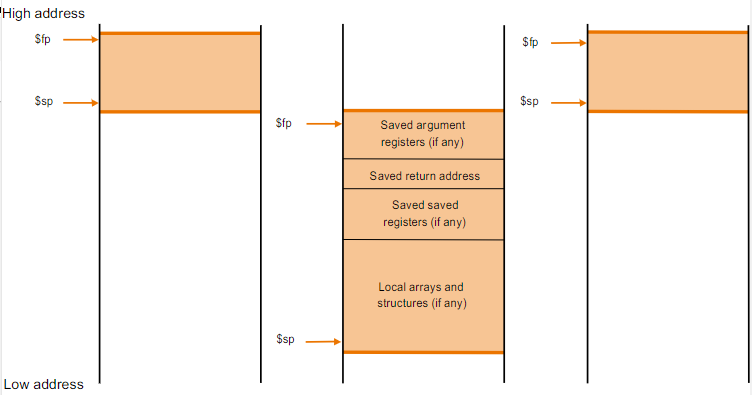
\includegraphics[width=0.489\textwidth]{CO3/Stack allocation before, during and after procedure call}
    \caption{Stack allocation before, during and after procedure call}
\end{figure}

\subsubsection{What is and what is not preserved across a procedure call}
\begin{table}[!htb]
    \centering
    \caption{across a procedure call}
    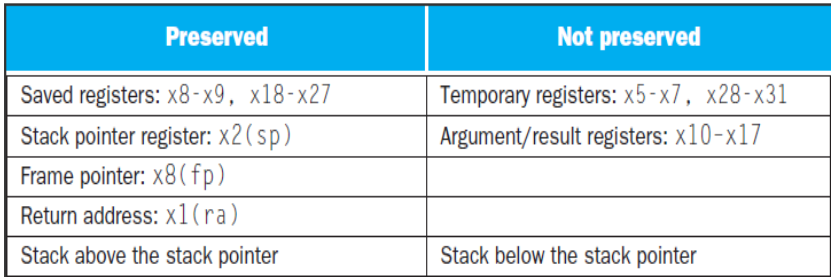
\includegraphics[width=0.489\textwidth]{CO3/across a procedure call}
\end{table}


\subsubsection{Memory Layout}


\begin{itemize}
    \item Text: program code
    \item Static data: global variables
    \item Dynamic data: heap
    \item Stack: automatic storage
    \item Storage class of C variables: 
    \begin{itemize}
        \item automatic
        \item static
    \end{itemize}
\end{itemize}

\begin{figure}[!htb]
    \centering
    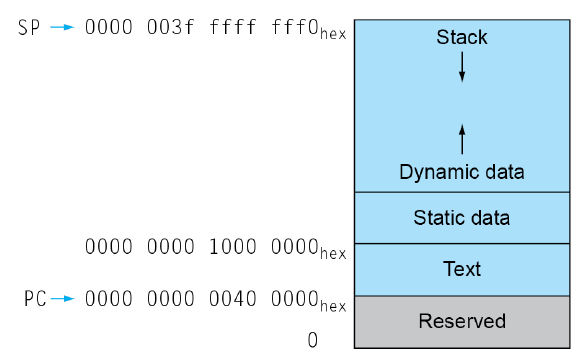
\includegraphics[width=0.309\textwidth]{CO3/Memory Layout}
    \caption{Memory Layout}
\end{figure}


\subsubsection{Local Data on the Stack}
Allocating Space for New Data on the Stack
\begin{itemize}
    \item Procedure frame/activation record: The segment of stack containing a procedure's saved registers and local variables. 
    \item Frame pointer
    \begin{enumerate}
        \item\small A value denoting the location of saved register and local variables for a given procedure
        \item\small Local data allocated by callee
    \end{enumerate}
    Used by some compilers to manage stack storage
\end{itemize}

\begin{figure}[!htb]
    \centering
    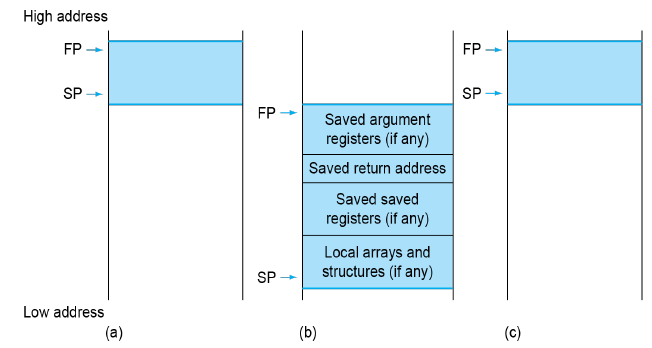
\includegraphics[width=0.479\textwidth]{CO3/Local Data on the Stack}
    \caption{Local Data on the Stack}
\end{figure}


\subsection{Communicating with Character Data}
Byte-encoded character sets
\begin{itemize}
    \item\small ASCII ( American Standard Code for Information Interchange ): 128 characters (95 graphic, 33 control)
    \item\small Latin-1: 256 characters (ASCII, +96 more graphic characters)
\end{itemize}



\subsubsection{Byte/Halfword/Word Operations}
RISC-V byte/halfword/word load/store
\begin{itemize}
    \item Load byte/halfword/word: Sign extend to 64 bits in rd
    \begin{lstlisting}[language={[x86masm]Assembler}]
lb rd, offset(rs1)
lh rd, offset(rs1)
lw rd, offset(rs1)
    \end{lstlisting}
    \item Load byte/halfword/word unsigned: 0 extend to 64 bits in rd
    \begin{lstlisting}[language={[x86masm]Assembler}]
lbu rd, offset(rs1)
lhu rd, offset(rs1)
lwu rd, offset(rs1)
    \end{lstlisting}
    \item Store byte/halfword/word: Store rightmost 8/16 /32 bits
    \begin{lstlisting}[language={[x86masm]Assembler}]
sb rs2, offset(rs1)
sh rs2, offset(rs1)
sw rs2, offset(rs1)
    \end{lstlisting}
\end{itemize}

\subsubsection{String Copy Example}
Compiling a string copy procedure ( Assume: base addresses for i -- x19, x's base -- x10, y's base -- x11 )
\begin{lstlisting}[language={c},title={C code: Y $\rightarrow$ X}]
void strcpy(char x[], char y[]){
    size_t i;
    i=0;
    while((x[i]=y[i])!='\0')
        i+=1;/* copy and test byte */
}
\end{lstlisting}

\begin{lstlisting}[language={[x86masm]Assembler},title={RISC-V assembly code}]
strcpy:
    addi sp, sp, 8
    sd s3, 0(sp)
    addi s3, zero, zero
L1: 
    add t0, s3, a1
    lbu t1, 0(t0)
    add t2, s3, a0
    sb t1, 0(t2)
    beq t1, zero L2
    addi s3, s3, 1
    jal zero, L1
L2:
    ld s3, 0(sp)
    addi sp, sp, 8
    jalr zero, 0(x1)
\end{lstlisting}
\begin{itemize}
    \item strcpy
    \begin{enumerate}
        \item adjust stack for 1 doubleword
        \item save x19
        \item i = 0
    \end{enumerate}
    \item L1
    \begin{enumerate}
        \item x5 = address of y[i]
        \item x6 = y [i]
        \item x7 = address of x[i]
        \item x[i] = y[i]
        \item if y[i] == 0 then exit
        \item i = i + 1
        \item next iteration of loop
    \end{enumerate}
    \item L2
    \begin{enumerate}
        \item restore saved old s3
        \item pop 1 double word from stack
        \item return
    \end{enumerate}
\end{itemize}

Optimization: Because strcpy is a leaf procedure, can allocate i to a temporary register s3/x18. 

For a leaf procedure, the compiler exhausts all temporary register, then use the registers it must save. 


\subsection{Addressing for 32-Bit Immediate and Addresses}
Wide Bit Immediate addressing:
\begin{itemize}
    \item most constants is short and fit into 12-bit field
    \item Set upper 20 bits of a constants in a register with load upper immediate (lui rd, constant)
\end{itemize}

\begin{lstlisting}[language={[x86masm]Assembler}]
    lui x19, 976
    \end{lstlisting}

\begin{figure}[!htb]
    \centering
    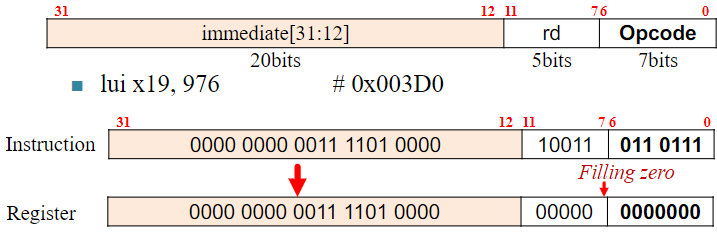
\includegraphics[width=0.479\textwidth]{CO3/U-type}
    \caption{instruction format (U-type)}
\end{figure}

\subsubsection{32-bit Constants}
Loading a 32-bit constant
\begin{align*}
    &0000\ 0000\ 0011\ 1101\ 0000\ 1001\ 0000\ 0000\\ 
    =&(976*16^3 + 2304=4000000)_{10}
\end{align*}

\begin{lstlisting}[language={[x86masm]Assembler},title={RISC-V code}]
lui s3, 976
addi s3, s3, 230
\end{lstlisting}
\begin{enumerate}
    \item 976 decimal = 0000 0000 0011 1101 0000 binary (The value of s3 afterward is: 0000 0000 0011 1101 0000 0000 0000 0000)
    \item 2304 decimal = 1001 0000 0000 binary
\end{enumerate}


\subsubsection{Branch Addressing}
Addressing in branches: 
\begin{itemize}
    \item Branch instructions specify opcode, two registers, target address. 
    \item Most branch targets are near branch, forward or backward. 
\end{itemize}
SB-type: 2000 = 0111 1101 0000
\begin{lstlisting}[language={[x86masm]Assembler}]
bne x10, x11, 2000
\end{lstlisting}
\begin{figure}[!htb]
    \centering
    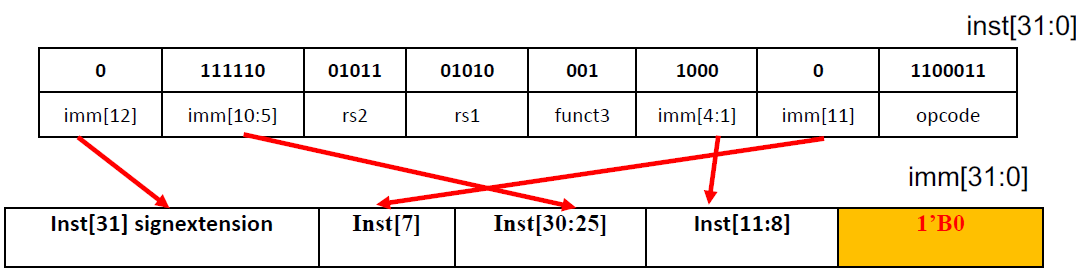
\includegraphics[width=0.479\textwidth]{CO3/Branch Addressing}
    \caption{Branch Addressing}
\end{figure}

\begin{align*}
    \text{Target address} &= \text{PC} + \text{Branch offset}\\
    &= \text{PC} + \text{immediate} \times 2
\end{align*}
\subsubsection{Jump  Addressing}
Jump and link (jal), target uses 20-bit immediate for larger range. 

UJ format: 2000=(0 00000000 0 111 1101 0000)
\begin{lstlisting}[language={[x86masm]Assembler}]
jal x0, 2000
\end{lstlisting}

% TODO P83补了

\subsubsection{Instructions Addressing and their Offset}
P85 学会看表

\subsection{Summary}
\subsubsection{RISC-V architecture}

\begin{table*}[hptb]
    \centering
    \caption{RISC-V operands}
    \label{RISC-V operands}
    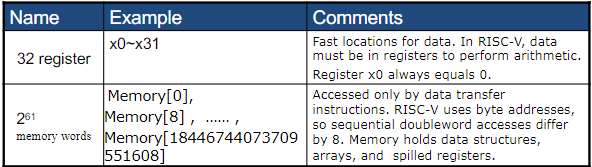
\includegraphics[width=0.88\textwidth]{CO3/RISC-V operands}
\end{table*}

\begin{table*}[hptb]
    \centering
    \caption{RISC-V register conventions}
    \label{RISC-V register conventions}
    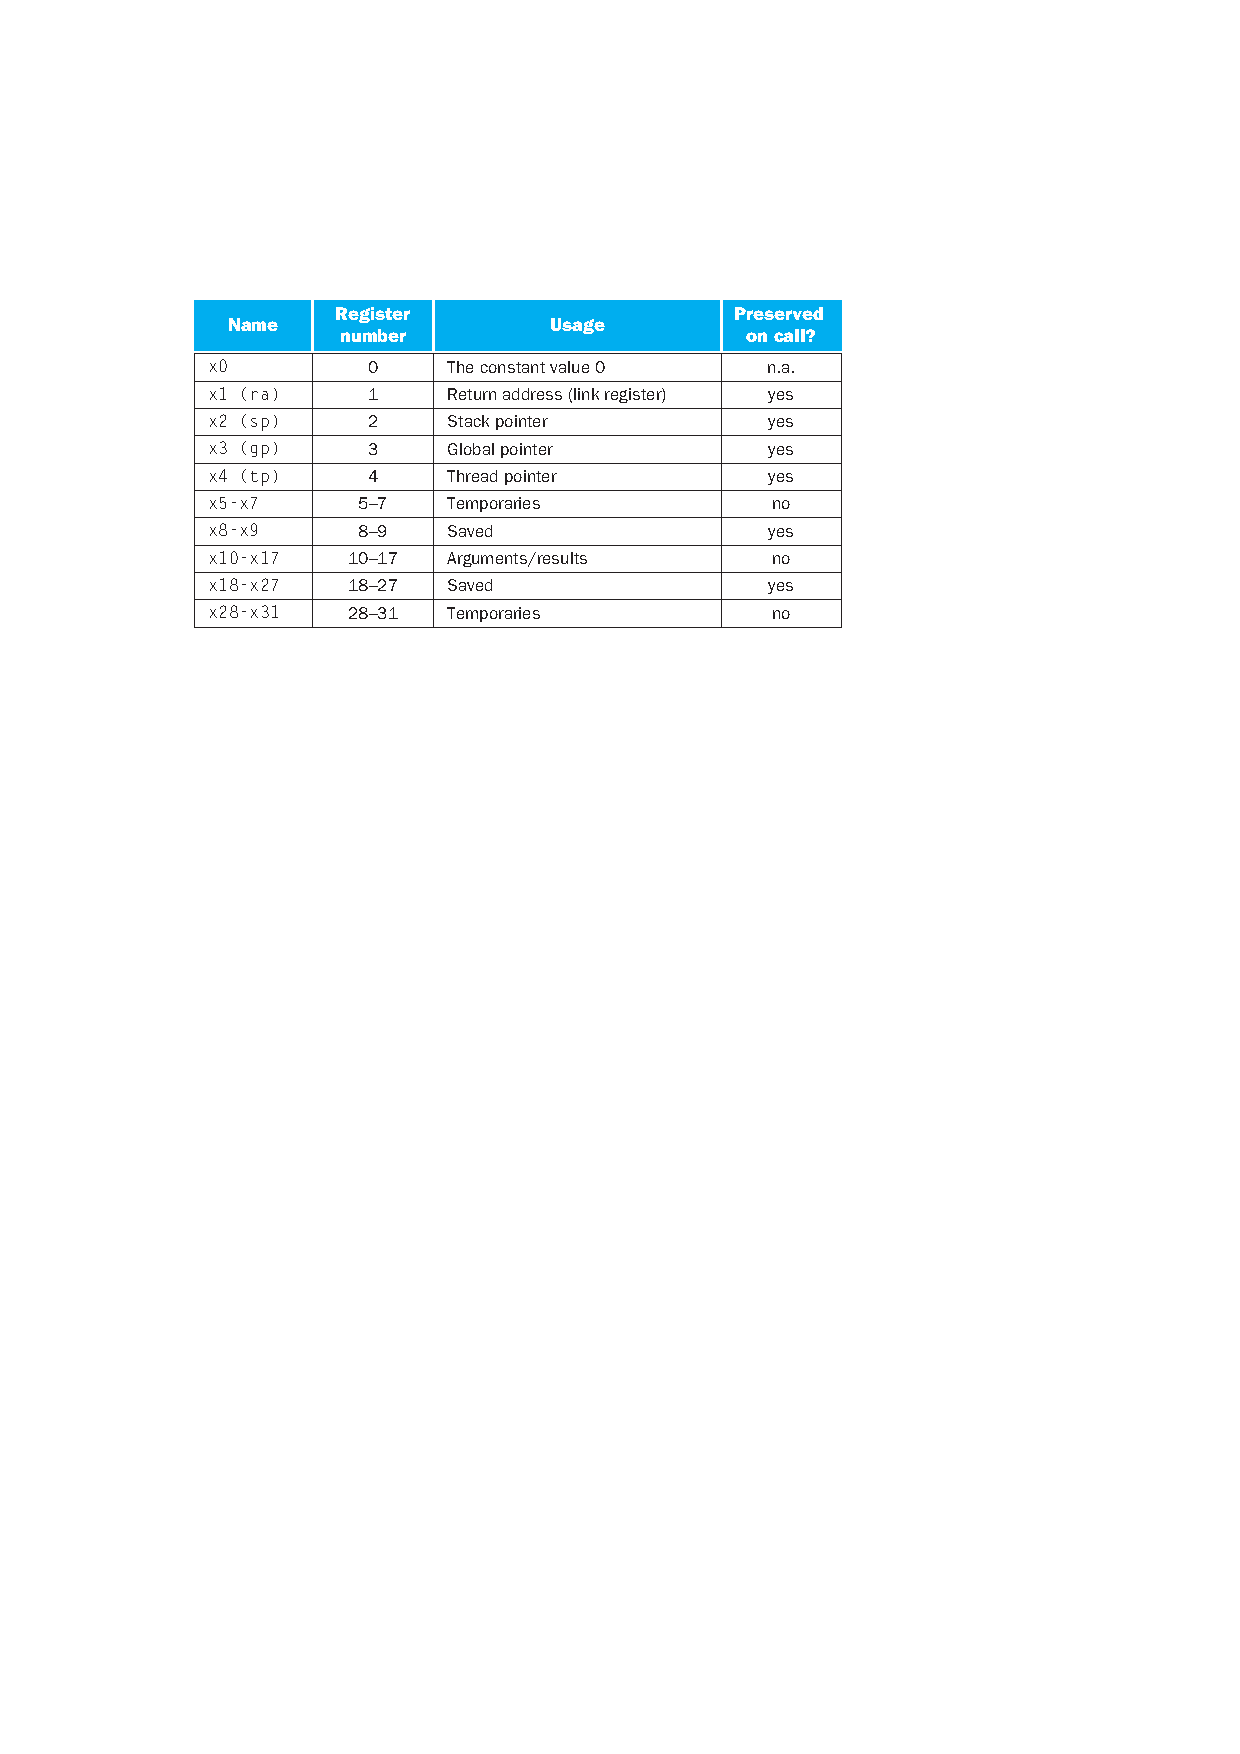
\includegraphics[width=0.618\textwidth]{CO3/RISC-V register conventions}
\end{table*}

\begin{table*}[hptb]
    \centering
    \caption{RISC-V Instruction Format}
    \label{RISC-V Instruction Format}
    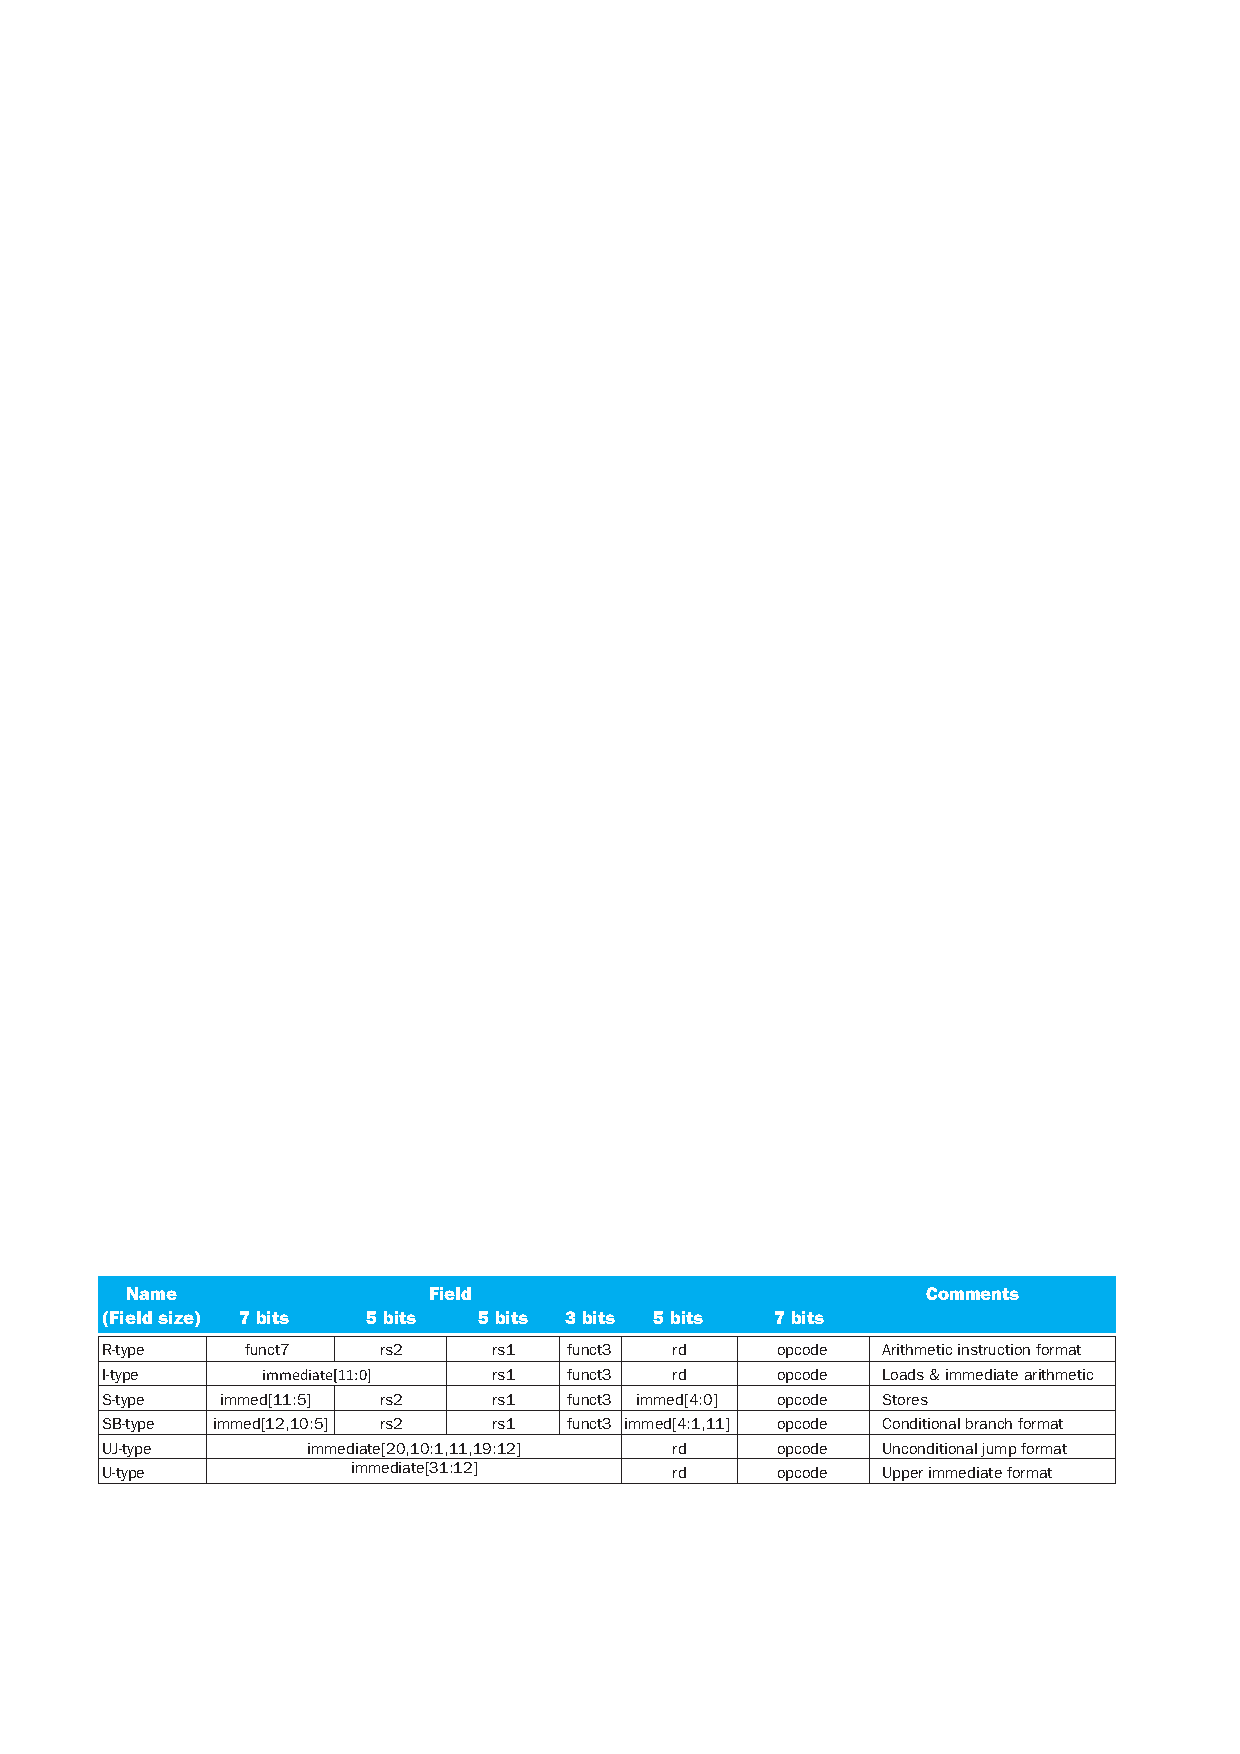
\includegraphics[width=0.88\textwidth]{CO3/RISC-V Instruction Format}
\end{table*}

\ref{RISC-V operands}
\ref{RISC-V register conventions}
\ref{RISC-V Instruction Format}



\subsubsection{RISC-V instruction encoding}
\begin{table*}[hptb]
    \centering
    \caption{RISC-V instruction encoding}
    \label{RISC-V instruction encoding}
    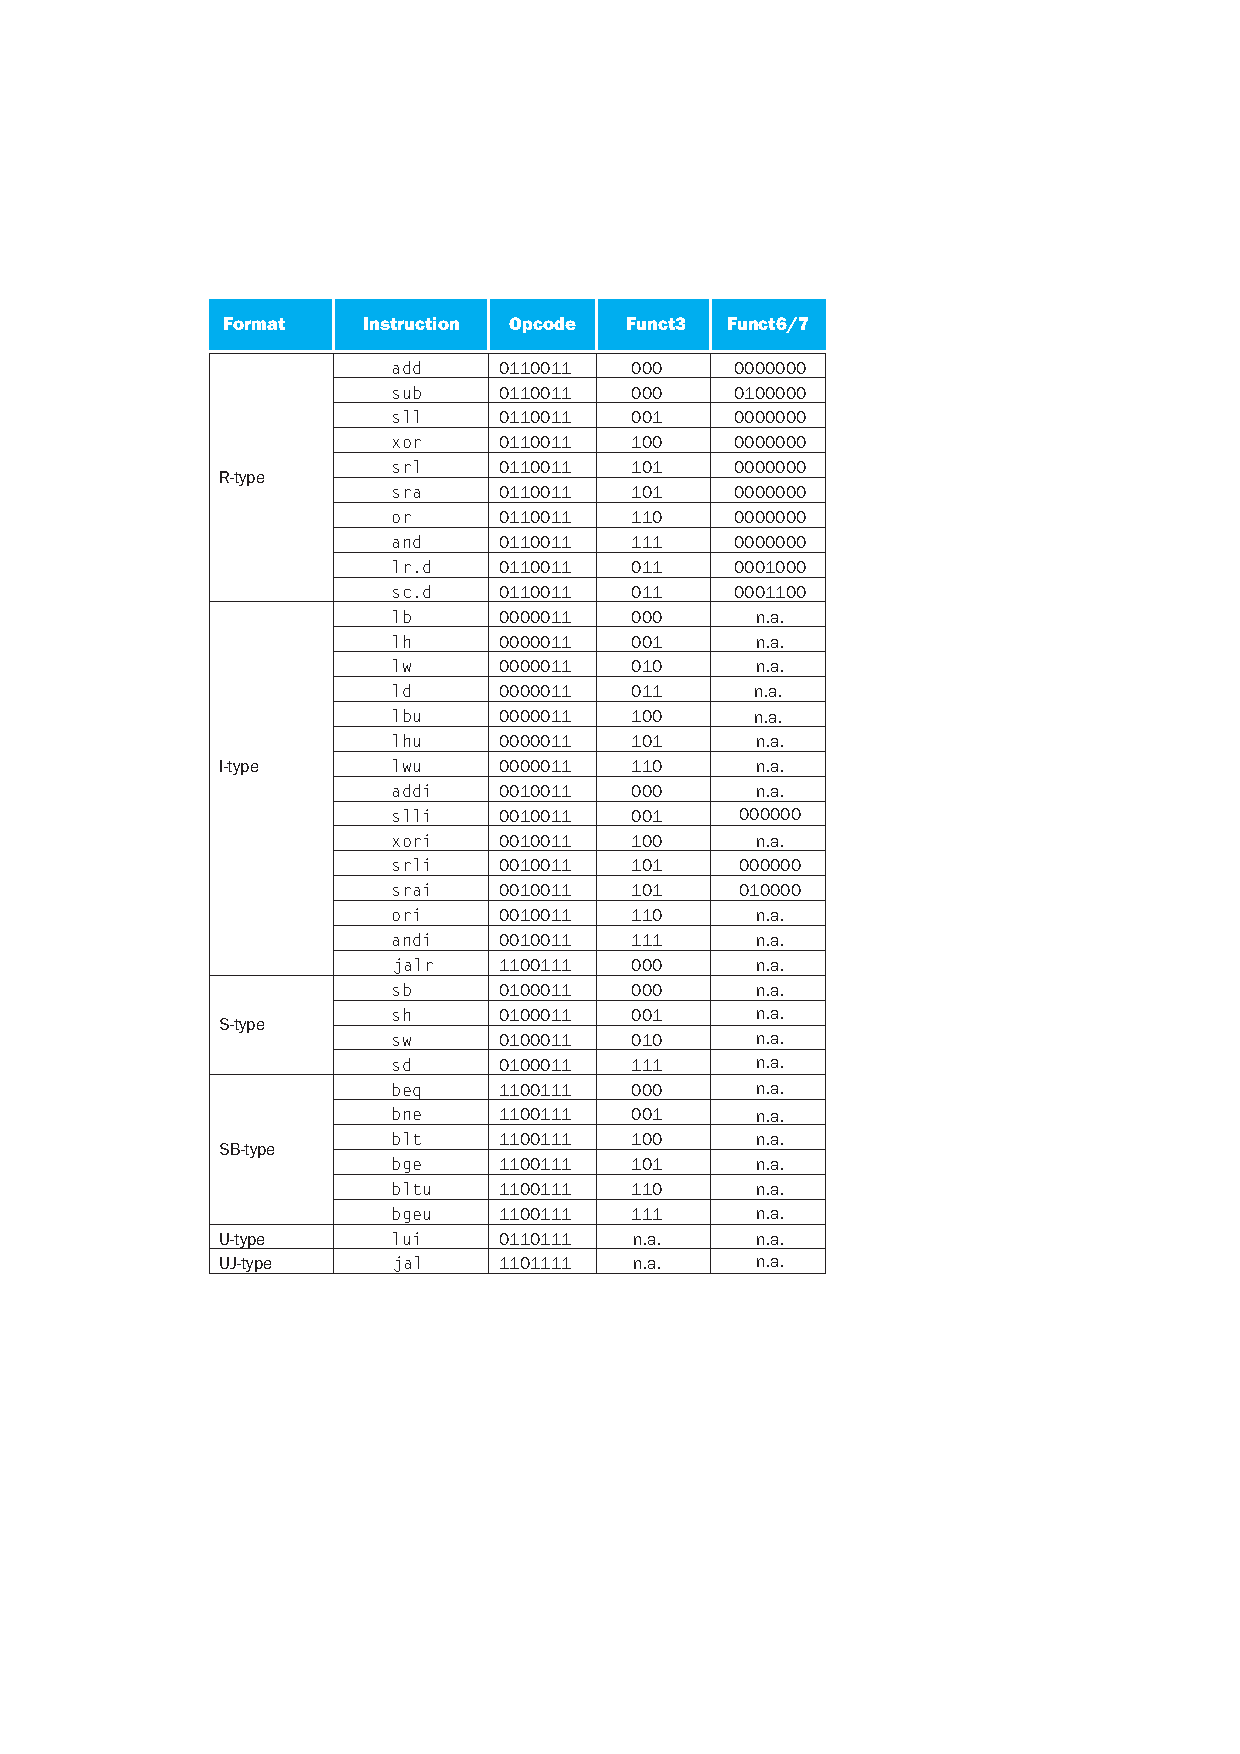
\includegraphics[width=0.618\textwidth]{CO3/RISC-V instruction encoding}
\end{table*}
\ref{RISC-V instruction encoding}

\subsubsection{RISC-V assembly language}
\begin{table*}[hptb]
    \centering
    \caption{RISC-V assembly language}
    \label{RISC-V assembly language}
    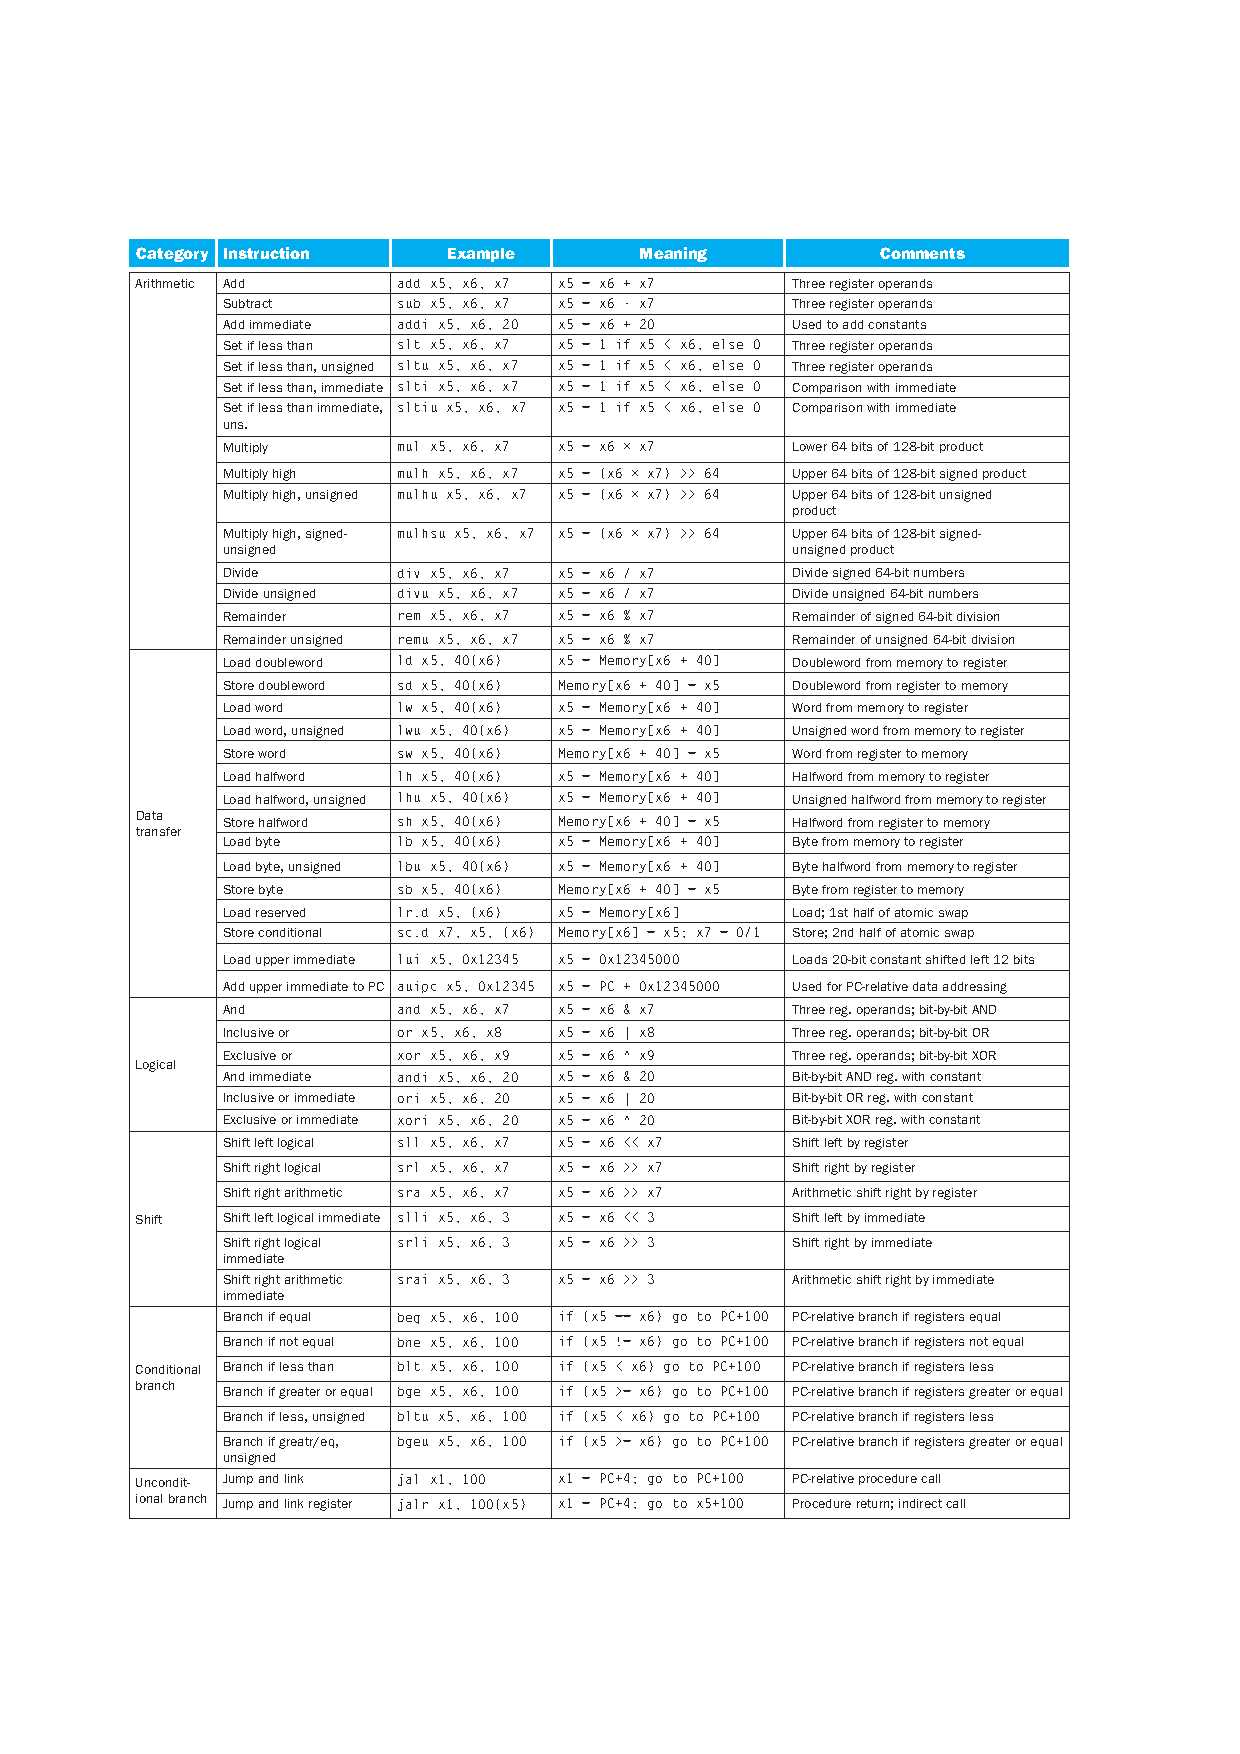
\includegraphics[width=0.86\textwidth]{CO3/RISC-V assembly language}
\end{table*}
\ref{RISC-V assembly language}


\subsection{Synchronization in RISC-V}
Two processors sharing an area of memory. Hardware support required. Could be a single instruction. (先读后写)

\begin{itemize}
    \item Load reserved: 
    \begin{lstlisting}[language={[x86masm]Assembler}]
lr.d rd,(rs1)
    \end{lstlisting}
    Load from address in rs1 to rd. Place reservation on memory address. 
    \item Store conditional:
    \begin{lstlisting}[language={[x86masm]Assembler}]
sc.d rd,(rs1),rs2
    \end{lstlisting}
    Store from rs2 to address in rs1. Succeeds if location not changed since the lr.d. Returns 0 in rd. Fails if location is changed. Returns non-zero value in rd
\end{itemize}

\subsubsection{atomic swap (to test/set lock variable)}
\begin{lstlisting}[language={[x86masm]Assembler},title={RISC-V assembly code}]
again:
    lr.d x10, (x20)
    sc.d x11, (x20), x23
    bne x11, x0, again
    addi x23, x10, 0
\end{lstlisting}
\begin{enumerate}
    \item x11 = status
    \item branch if store failed
    \item x23 = loaded value
\end{enumerate}

\subsubsection{lock}
\begin{lstlisting}[language={[x86masm]Assembler},title={RISC-V assembly code}]
    addi x12, x0, 1
again:
    lr.d x10, (x20)
    bne x10, x0, again
    sc.d x11, (x20), x12
    bne x11, x0, again
\end{lstlisting}
\begin{enumerate}
    \item copy locked value
    \item read lock
    \item check if it is 0 yet
    \item attempt to store
    \item branch if fails
\end{enumerate}

\begin{lstlisting}[language={[x86masm]Assembler},title={RISC-V assembly code}]
Unlock: 
    sd x0, 0(x20)
\end{lstlisting}
free lock

\subsection{Translating and starting a program}
\begin{figure}[!htb]
    \centering
    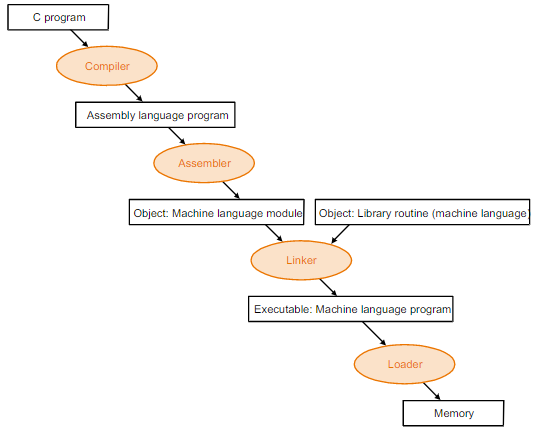
\includegraphics[width=0.489\textwidth]{CO3/Translating a program}
    \caption{Translating a program}
\end{figure}

\subsubsection{Producing an Object Module}
Assembler (or compiler) translates program into machine instructions. Provides information for building a complete program from the pieces:
\begin{itemize}
    \item Header: described contents of object module
    \item Text segment: translated instructions
    \item Static data segment: data allocated for the life of the program
    \item Relocation info: for contents that depend on absolute location of loaded program
    \item Symbol table: global definitions and external refs
    \item Debug info: for associating with source code
\end{itemize}

\begin{table}[!htb]
    \centering
    \caption{Producing an Object Module}
    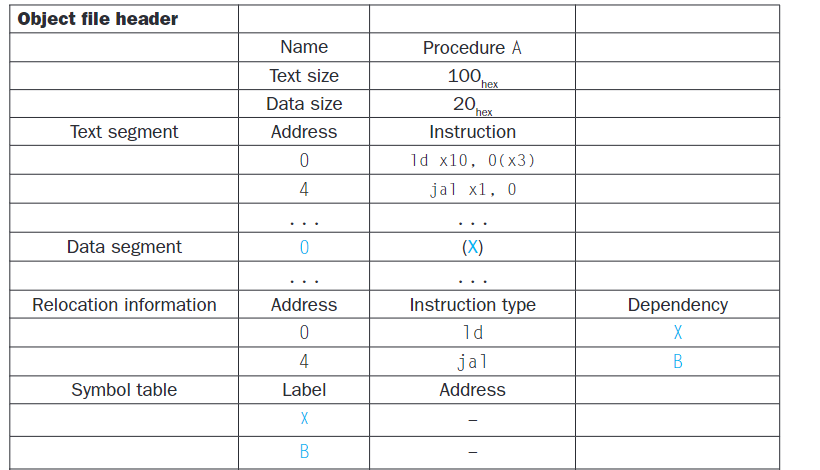
\includegraphics[width=0.479\textwidth]{CO3/Producing an Object Modul}
\end{table}


\subsubsection{Link}
Object modules(including library routine) $\leftarrow$ executable program. 
\begin{enumerate}
    \item Place code and data modules symbolically in memory
    \item Determine the addresses of data and instruction labels
    \item Patch both the internal and external references (Address of invoke)
\end{enumerate}

\begin{figure}[!htb]
    \centering
    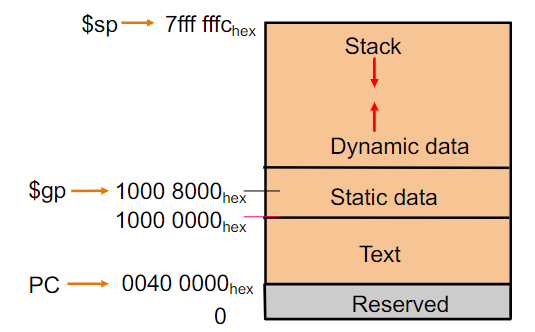
\includegraphics[width=0.309\textwidth]{CO3/Link}
    \caption{Link}
\end{figure}


\subsubsection{Loading a Program}
Load from image file (镜像文件) on disk into memory
\begin{enumerate}
    \item Read header to determine segment sizes
    \item Create virtual address space
    \item Copy text and initialized data into memory. Or set page table entries so they can be faulted in
    \item Set up arguments on stack
    \item Initialize registers (including sp, fp, gp)
    \item Jump to startup routine
    \begin{itemize}
        \item Copies arguments to x10, ... and calls main
        \item When main returns, do exit syscall
    \end{itemize}
\end{enumerate}

\subsubsection{Dynamic Linking}
Only link/load library procedure when it is called. 
\begin{itemize}
    \item Requires procedure code to be relocatable
    \item Avoids image bloat caused by static linking of all (transitively) referenced libraries
    \item Automatically picks up new library versions
\end{itemize}

\subsubsection{Lazy Linkage}
\begin{figure}[!htb]
    \centering
    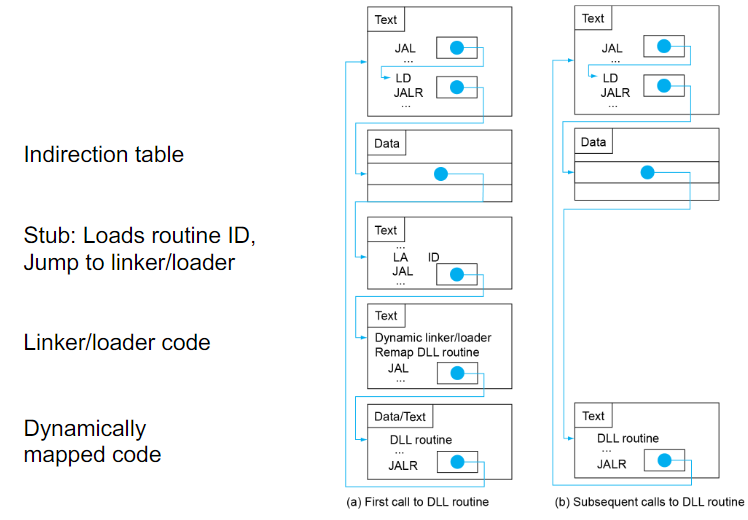
\includegraphics[width=0.309\textwidth]{CO3/Lazy Linkage}
    \caption{Lazy Linkage}
\end{figure}


\subsection{A C Sort Example To Put it All Together}
Three general steps for translating C procedures
\begin{enumerate}
    \item Allocate registers to program variables
    \item Produce code for the body of the procedures
    \item Preserve registers across the procedures invocation
\end{enumerate}

P104

\subsection{Arrays versus Pointers}
e.g. P111

\subsubsection{Comparison of Array vs Pointers}
P112

% TODO 补笔记
